% BÀI TOÁN HÌNH HỌC - BAI_HINH_19 (TRÍCH ĐỀ 19)
\begin{ex}
Cho tam giác ABC nhọn (AB < AC) nội tiếp đường tròn (O). Các đường cao CD và BK cắt nhau tại trực tâm H của tam giác ABC.
	\begin{enumerate}
		\item[a)] Chứng minh 4 điểm A, D, H, K nằm trên một đường tròn.
		\item[b)] Kẻ đường kính AN, chứng minh: BHCN là hình bình hành. Gọi M là trung điểm của BC, chứng minh OM = $\frac{1}{2}$AH và $\widehat{ABK} = \widehat{OCB}$.
	\end{enumerate}
\loigiai{
{
	\begin{center}
		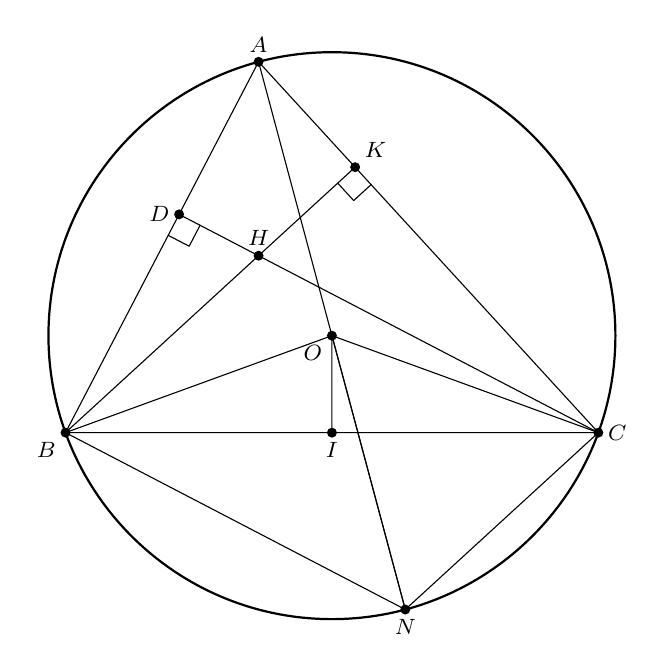
\begin{tikzpicture}[line join = round, line cap=round,>=stealth,font=\footnotesize,scale=1.2]
			\usetikzlibrary{calc,angles,quotes}
			% Def
			\def\r{3}
			
			% Coordinates
			\coordinate (O) at (0,0);
			\coordinate (A) at (105:\r);
			\coordinate (B) at (-160:\r); % or (200:\r)
			\coordinate (C) at (-20:\r);  % or (340:\r)
			
			% N such that O is midpoint of AN
			% N is A reflected through O, so N = -A (vector)
			% or N has angle of A + 180 deg
			\coordinate (N) at (105+180:\r); % or (-75:\r) or (285:\r)
			
			% I is midpoint of BC
			\coordinate (I) at ($ (B)!0.5!(C) $);
			
			% D is projection of C onto AB
			\coordinate (D) at ($ (A)!(C)!(B) $);
			
			% K is projection of B onto AC
			\coordinate (K) at ($ (A)!(B)!(C) $);
			
			% H is intersection of CD and BK (orthocenter of triangle ABC)
			% If O is circumcenter (which it is), H = A+B+C (vector sum from O)
			\coordinate (H) at ($ (A) + (B) + (C) $);
			
			% Draw
			% Draw circle (O,r)
			\draw[thick] (O) circle (\r);
			
			% Draw paths A-B-N-C-A-N-O-B-C-D-H-K-B
			\draw (A) -- (B) -- (N) -- (C) -- (A); % Quadrilateral ABNC and diagonal AC (actually CA)
			\draw (A) -- (N); 
			\draw (N) -- (O) -- (B);
			\draw (B) -- (C)--(O)--(I); 
			\draw (C) -- (D) -- (H) -- (K) -- (B);
			
			% Fill points
			\fill (O) circle (1.5pt);
			\fill (A) circle (1.5pt);
			\fill (B) circle (1.5pt);
			\fill (C) circle (1.5pt);
			\fill (N) circle (1.5pt);
			\fill (I) circle (1.5pt);
			\fill (D) circle (1.5pt);
			\fill (K) circle (1.5pt);
			\fill (H) circle (1.5pt);
			
			% Node points (old style)
			\node[below left] at (O) {$O$};
			\node[above] at (A) {$A$};
			\node[below left] at (B) {$B$};
			\node[right] at (C) {$C$}; 
			\node[below] at (N) {$N$}; 
			\node[below] at (I) {$I$}; % Adjusted for I on negative y-axis
			\node[left] at (D) {$D$};
			\node[above right] at (K) {$K$}; 
			\node[above] at (H) {$H$}; % Adjusted for H in Q2
			
			% Ky hieu goc vuong (old style)
			% CD is altitude to AB, so angle CDB or CDA is 90. C-D-B
			\pic[draw, angle radius=3mm]{right angle = B--D--C};
			% BK is altitude to AC, so angle CKB or AKB is 90. C-K-B
			\pic[draw, angle radius=3mm]{right angle = C--K--B};
			
		\end{tikzpicture}
		
	\end{center}
}
\end{ex}
